\chapter{Visual recognition}
The pictures accompanying the posts usually help a lot in determining the emotion of the user. For instance, happy photos might contain landscapes with the sun or a beach while sad ones might have really dark colors. To analyse the images, we'll use convolutional neural networks, which achieve state-of-the-art performances in many visual recognition tasks. First we'll explain how they work and then we'll dive into the architecture we've used for deep sentiment analysis.
%%%%%%%%%%%%%%%%%%%%%%%%%%%%%%%%%%%%%%%%%%%%%%%%%%%%%%%%%%%%
%%%%%%%%%%%%%%%%%%%%  NEW SECTION   %%%%%%%%%%%%%%%%%%%%%%%%
%%%%%%%%%%%%%%%%%%%%%%%%%%%%%%%%%%%%%%%%%%%%%%%%%%%%%%%%%%%%
\section{Convolutional neural networks}
A convolutional neural networks, often called ConvNets, can be seen as a simulation of the human visual cortex, that is to say an aggregation of plenty of receptive fields. (some illustrations might be helpful here)

\subsection{Convolutional layer}
Take an image of dimension $(h,w,3)$ with $h$ the height, $w$ the width and 3 representing the number of channels (red, blue, green). If you simply flatten that image and transform it into a vector of size $h\times h \times 3$ and feed that vector to a neural network, you'll get not-so-good results as you've thrown away all the spatial information. Convolutions extract that spatial information and work the following way:
\begin{itemize}
\item Each convolution is described by a filter F of size $(f, f, 3)$, $f$ usually being in the range $[1,13]$.
\item Position the filter on the upper left of the image and element-wise multiply with the filter, then sum those numbers to obtain a raw number.
\item Slide across the image, one pixel at a time horizontally and vertically, and repeat the previous operation.
\end{itemize}

\begin{figure}
\begin{subfigure}[t]{.5\textwidth}
  \vskip 0pt
  \centering
  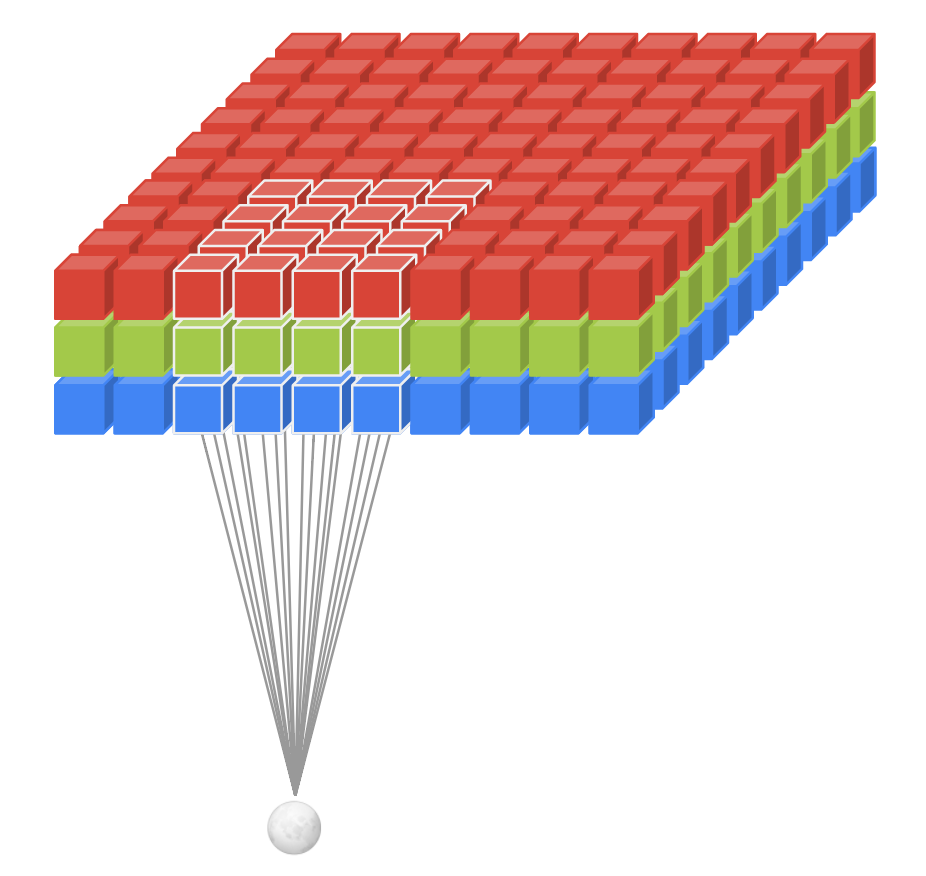
\includegraphics[width=.8\linewidth]{Images/conv1.png}
  \caption{One operation of convolution}
\end{subfigure}
\begin{subfigure}[t]{.5\textwidth}
  \vskip 0pt 
  \centering
  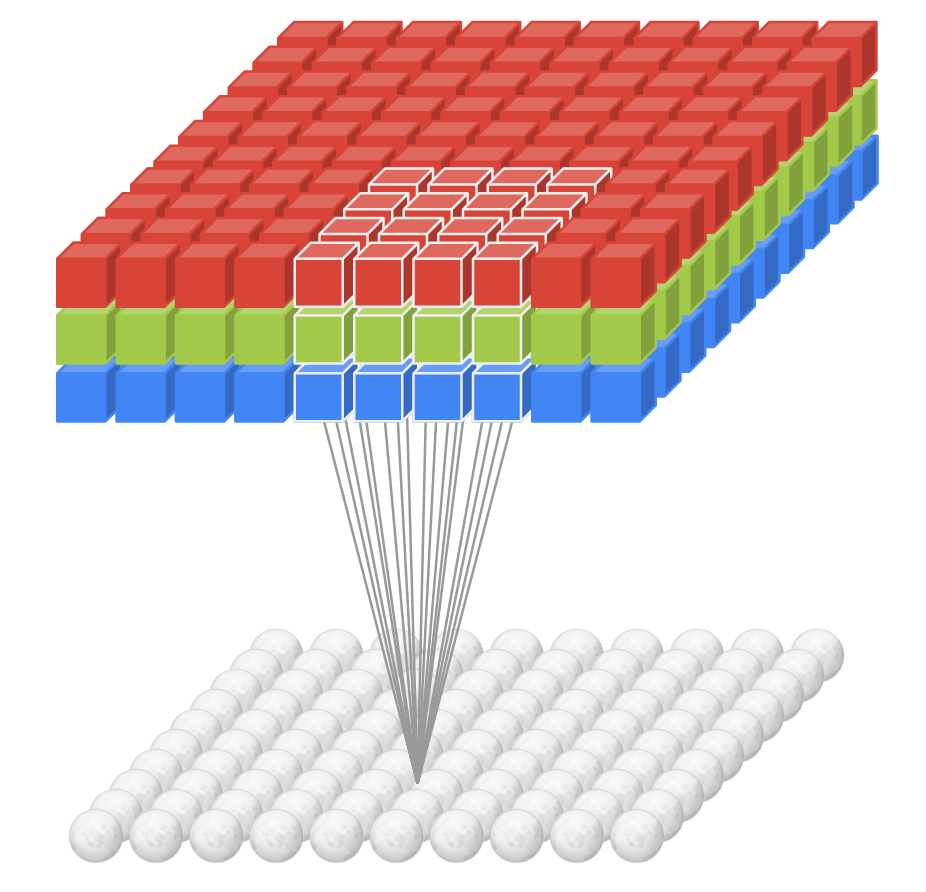
\includegraphics[width=.8\linewidth]{Images/conv2.png}
  \caption{The result of the convolution}
\end{subfigure}
\caption{A convolution, each neuron been a `receptive field' \cite{gorner}}
\end{figure}

By sliding through the image, you would get a new matrix of dimension $(h_{new}, w_{new},1)$, with $h_{new}=h-f+1$ and $w_{new}=w-f+1$. However, we usually don't want to reduce the size of our input image that fast, as we usually have several convolutions. To ensure that the image has the same size, zero-padding is used: we add $p$ zeros to the borders of the input image to preserve the spatial size of the input. With zero-padding, $h_{new}$ becomes: $h_{new} =  h + 2p - f + 1$, and we want that $h_{new}$ equals $h$:
\begin{equation}
h + 2p - f + 1 = h
\end{equation}
Therefore, $p=\frac{f-1}{2}$.

A convolution extract information about the image such as edges or blotches of some color (Figure \ref{conv-ex}). The grayscale and edges filters were hardcoded but in a ConvNet setting, the weights of the filter F are learned through optimising a loss function -- in our case, a metric measuring how accurate our predictions of the emotions are. The network will learn weights that will detect features that will be most relevant to our specific task. Most of the time, more than a single convolution are used: just repeat that operation $d$ (the depth) times, to create a new tensor of dimension $(h,w,d)$. We can then apply convolutions on that new image. First layers will recognise simple features such as edges or aggregation of colors, and deeper layers might activate on faces, wheels and so on.

\begin{figure}
\centering
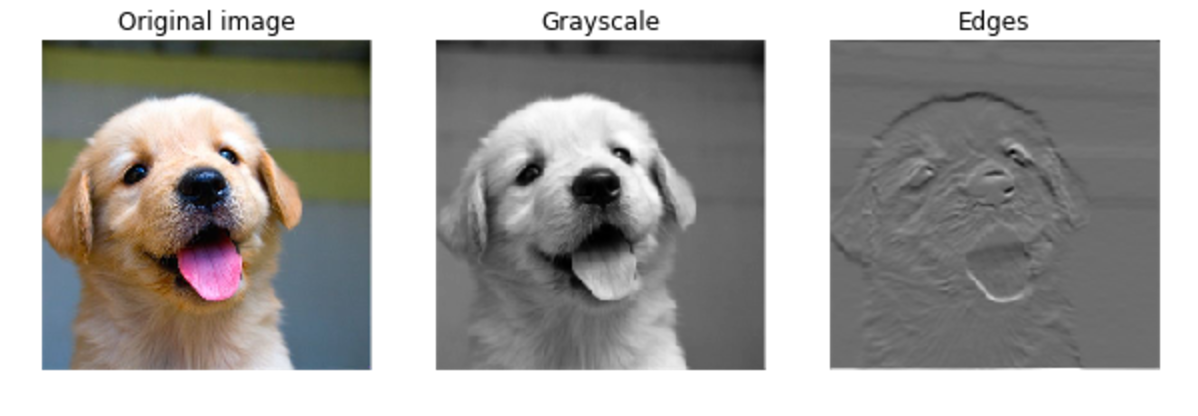
\includegraphics[width=0.8\textwidth]{Images/conv_ex.png}
\caption{Examples of convolution}
\label{conv-ex}
\end{figure}

\subsection{ReLU layer}
Stacking convolutions is nice, but as it is, we are only creature features that are linearly dependent of the input pixels: we could replace all the convolutions with a single matrix multiplication. In order to learn more interesting functions, we have to add non-linearities. Historically, the popular choice was the sigmoid function defined as:
\begin{equation}
\text{sigmoid}(x) = \frac{1}{1+e^{-x}}
\end{equation}

\begin{figure}[H]
\centering
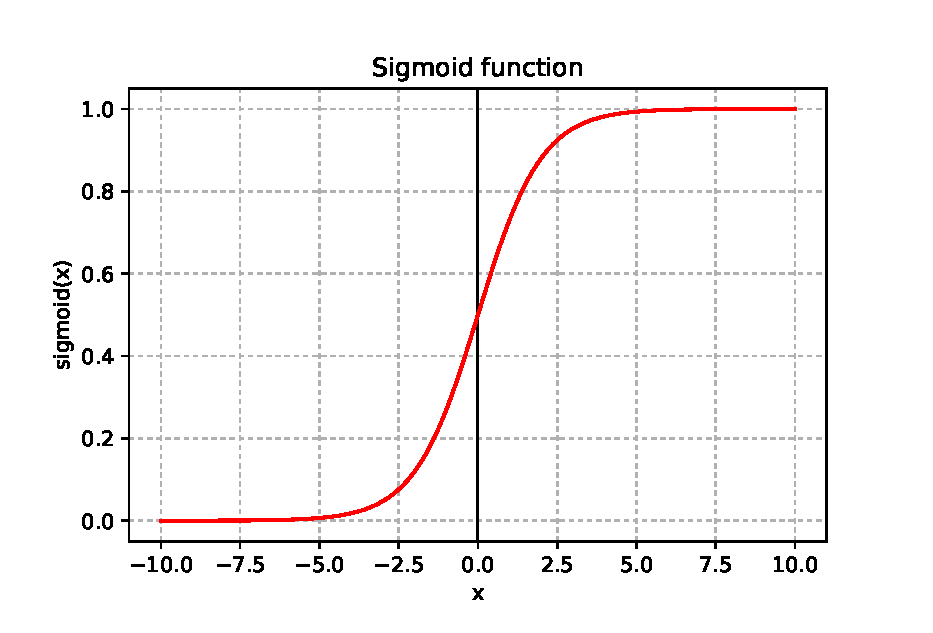
\includegraphics[width=0.75\textwidth]{Images/sigmoid.eps}
\caption{Sigmoid function}
\end{figure}

The sigmoid function is the simplest function having values between 0 and 1 mimicking the biological neurons `firing' to their inputs. However, when the network is learning to minimise a loss function through backpropagation, the gradients tend to vanish to zero as the sigmoid's derivative goes to zero for high negative and positive values. The most popular choice is now the Rectified Linear Unit (ReLU) defined as:
\begin{equation}
\text{ReLU}(x) = \text{max}(0,x)
\end{equation}

\begin{figure}[H]
\centering
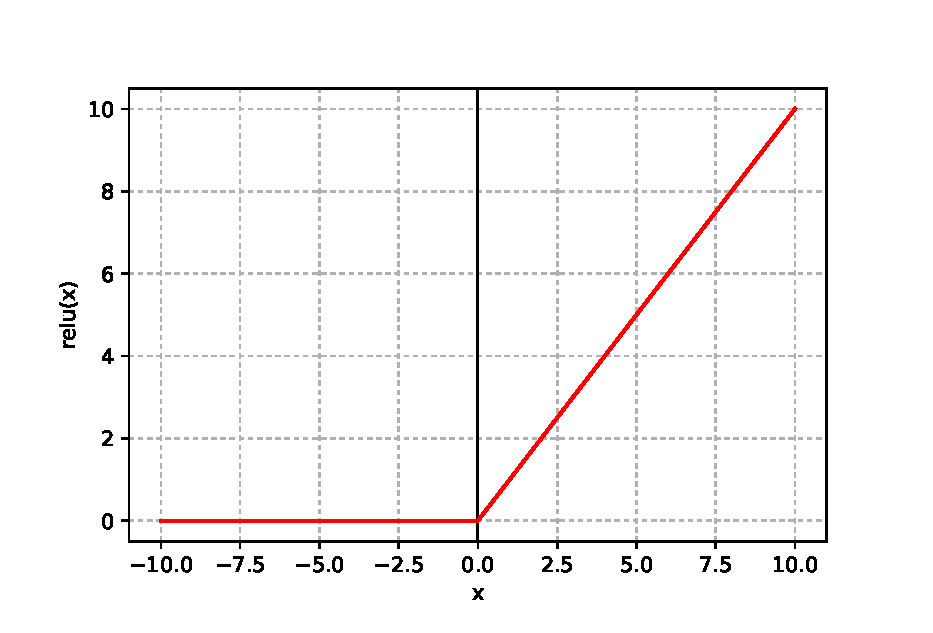
\includegraphics[width=0.75\textwidth]{Images/relu.eps}
\caption{Sigmoid function}
\end{figure}

The ReLU's gradient is non-saturating for highly excited neurons which turns out to be a nice property to learn faster. In the network, each layer of convolution is followed by a ReLU layer, that simply applies the function $\text{max}(0,x)$ to each neuron.

\subsection{Pooling layer}
After a few iterations of convolutions, inserting pooling layers in-between convolutional layers might be a good idea to control the spatial complexity of the network. More concretely, what is most used in practice is the 2x2 max-pooling:
\begin{itemize}
\item Pick a channel among the $d$ ones.
\item Position yourself on the top-left 2x2 square of the image and take the max.
\item Repeat by sliding through the image vertically and horizontally with a stride (step) of 2.
\end{itemize}

\begin{figure}
\centering
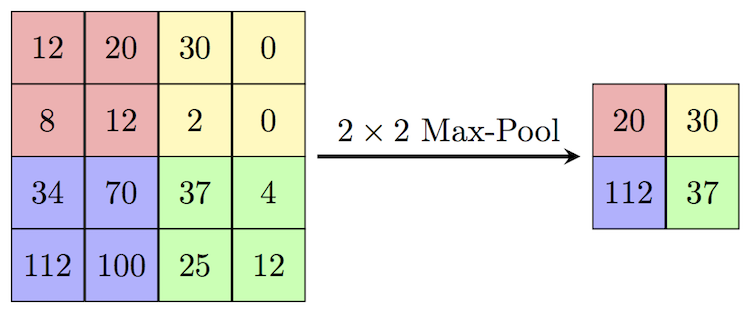
\includegraphics[width=0.8\textwidth]{Images/maxpool.png}
\caption{Max pooling \cite{camb-spark}}
\end{figure}

After applying max pooling to each channel, the resulting image's dimension is $(\frac{h}{2}, \frac{w}{2}, d)$ and we have discarded 75\% of the neurons (as in each max-pool operation, we only keep the maximum neuron among the fours), effectively reducing the number of parameters and controlling overfitting. Pooling is also useful to create translation-invariant features.

\subsection{An example of ConvNet}
Here is an example of a convolutional neural network with an input image of size $(100, 100, 3)$:

\begin{figure}[H]
\centering
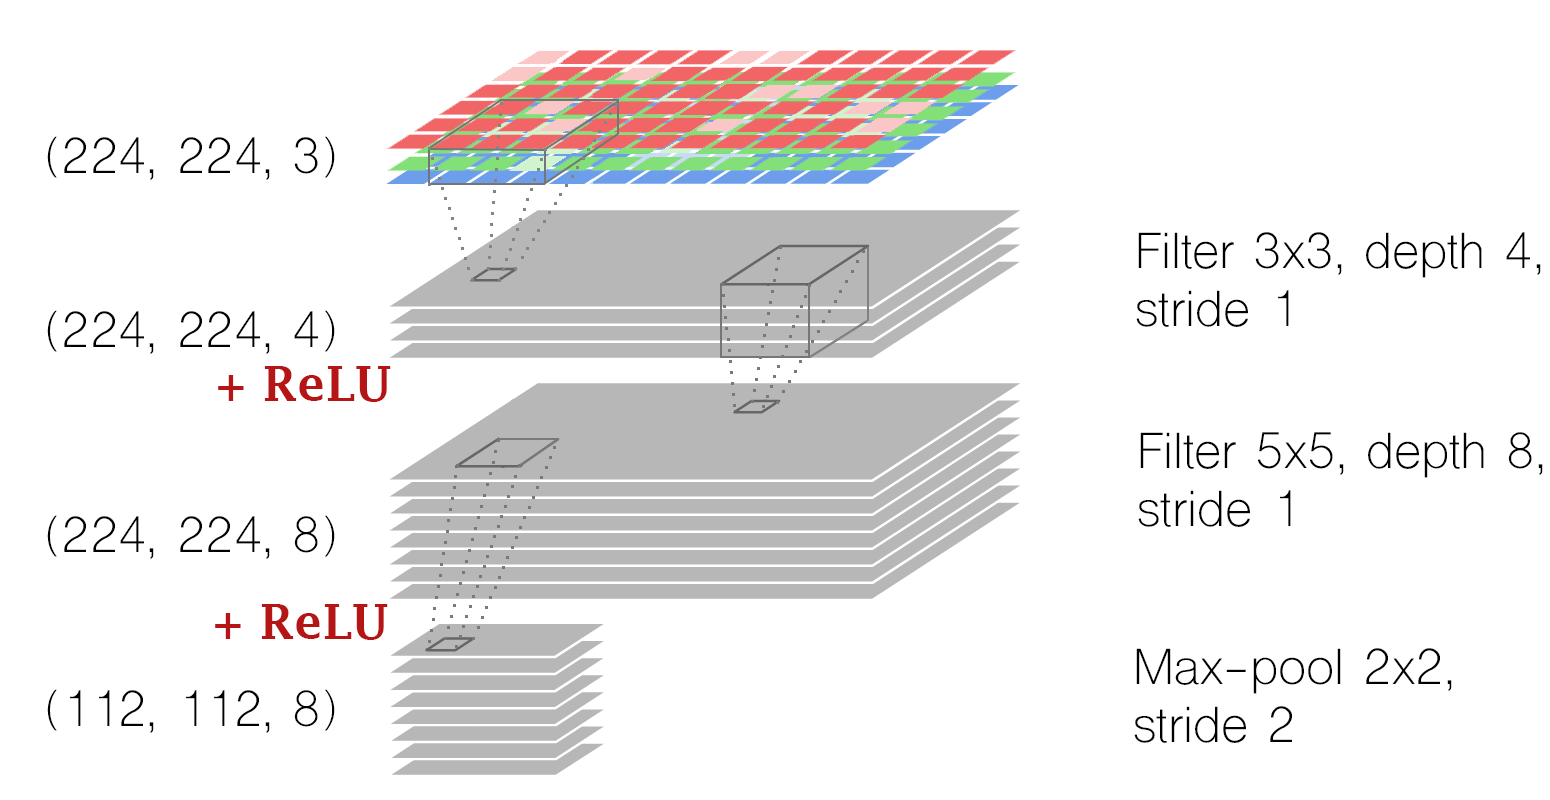
\includegraphics[width=0.8\textwidth]{Images/conv_archi.png}
\caption{An architecture of a neural network \cite{gorner}}
\end{figure}

\begin{itemize}
\item A first convolution with a filter of size $3\times3$ is applied, with depth 4, stride 1 and zero-padding of 1.
\item A ReLU layer.
\item A second convolution with a filter of size $5\times5$ is applied, with depth 8, stride 1 and zero-padding of 2.
\item A ReLU layer.
\item Max-pooling of size $2\times2$ with stride 2, reducing the height and width by 2.
\end{itemize}

After the last operation, the neurons are reshaped into a vector that can be fed to the traditional fully-connected layers of neural networks.

\subsection{Deep convolutional networks}
Best results are achieved using deep convolutional networks, that is to say by stacking many layers of convolutions, ReLU, max-pool. But what exactly is `many'? Let us have a look at the main Computer Vision competition: ImageNet Large Scale Visual Recognition (ILSVR).
\begin{enumerate}
\item \textbf{AlexNet} \cite{alexnet}: The first popular convolutional network, developed by Alex Krizhevsky, Ilya Sutskever and Geoffrey Hinton, that outperformed the other competitors at the ILSVR 2012 by a large margin: top-5 error of 16\% compared to the runner-up with 26\%. AlexNet has 5 convolutional layers (followed by ReLU), 3 max-pool layers and 3 fully-connected layers, producing a 8-layer deep network (not counting the max-pooling as it doesn't have any parameters).
\item \textbf{GoogLeNet} (also known as Inception)\cite{googlenet}: This is the winner of the ILSVR 2014 with a top-5 error of 6.7\% . This architecture used the `Inception Module' which allowed to drastically reduce the number of parameters: from 60M for AlexNet to 4M for GoogLeNet. 
\end{enumerate}


